\section{Grasping \& Manipulation System}
\label{sec:manip}
%
In this section we present an integrative approach for grasp representation and motion
generation. The main idea is to provide a functional representation of grasps as intervals in task
space, which allows redundancy in the gripper pose prior to executing the grasp. Subsequently, we
leverage the obtained redundancy to generate reactive manipulator motions by formulating a
representation of the corresponding tasks in the prioritized motion control framework proposed by
Kanoun et al.~\cite{Kano11}.
%
\subsection{Challenges in Autonomous Grasping}
\label{subsec:Grasping_challenges}
%
In current autonomous grasping systems~\cite{Bere07, Srin10, Krug14a}, grasp planning and
manipulator motion planning are usually seen as independent sub-problems~\cite{Dian10}. A database
storing object models together with sets of pre-computed grasps is used to find suitable gripper
poses/configurations~\cite{Mill04, Gold11, Krug14a}. In the online stage, sampling based
planners~\cite{LaVa06} attempt to generate valid trajectories for the pre-planned grasps, which are
executed in a feasible-first manner~\cite{Bere07}. During the execution phase, such approaches
necessitate many futile motion planning attempts, which often incurs significant time delays since
sampling based planners suffer from the curse of dimensionality. Also, while being able to solve
complicated planning problems if given enough time, these planners do not scale well to
geometrically simple scenarios and they are ill suited to incorporate contact events with the
environment which is a prerequisite for any grasping/manipulation application.

Using control to exploit manipulator redundancy has long been in the focus of research~\cite{Sici91,
  Sent10}. In this line of thought, opposed to define a set of discrete grasp poses, Gienger et
al.~\cite{Gien08a, Gien08b} learn a manifold of feasible grasps for an object and use an
attractor-based control scheme to reach the corresponding volume in the task space. Another approach
to address motion planning and motion control simultaneously, is to formulate a hierarchical stack
of equality tasks which are represented as task functions~\cite{Sams91}. Lower-ranked tasks are then
solved in the null-space of tasks with higher priority~\cite{Sici91, Sent10}. A major step forward
in this direction was achieved by Kanoun et al.~\cite{Kano11}, who extended the approach to include
inequality tasks which significantly increases the expressiveness of the method. Recent advancements
include the extension to dynamic control~\cite{Saab13} and an efficient solution algorithm for the
underlying optimization problem~\cite{Esca14}.
%
\subsection{Object Detection}
\label{subsec:obj_det}
%
A typical commissioning scenario in a warehouse environment generally involves as a first step the
identification and localization of an object targeted for picking. There are however many
application scenario specific factors to consider when designing an object detection system for this
task. For example: a single pallet may hold a homogeneous or a heterogeneous set of objects; objects
may be stored in boxes and equipped with barcodes; objects may be stored on shelves, pallets, or
simply piled up. For this work, we assumed a simple scenario where objects of the same type are
stored on a single pallet. As shown in Fig.~\ref{fig:robot}, the gripper of the APPLE system is
equipped with a structured light depth sensor\footnote{\url{http://structure.io/}}. We use the 3D
point clouds generated by the sensor as an input for a simple object detection module which
identifies clusters of points matching our expected object models. The object detection module was
implemented using the Point Cloud Library (PCL)\footnote{\url{http://pointclouds.org/}} following
the simple procedure summarized in Algorithm~\ref{alg:obj}.
%http://pointclouds.org/
\begin{algorithm}[t!]
%\DontPrintSemicolon
\SetKwInOut{Input}{input}
\SetKwInOut{Output}{output}
\Input{Pointcloud $P$, kinematic model $K$, joint positions $\mbm{j}$}
\Output{Target cluster $T$}
Transform $P$ into world coordinates using $K,\mbm{j}$\;
\While {target plane not found} {
    Extract plane $\mbm{n},d$ from $P$ using RANSAC\;
    \If{$\mbm{n}\mbm{z} < \cos{\alpha}, abs(d-h_{pallet}) < e_{pallet}$}{target plane found\;}
    \Else{ Remove inliers and iterate. If points in $P$ less than $20\%$ of original points, report failure\;}
}
Extract oriented bounding box (OBB) of plane inliers\;
Extract points inside OBB and height in $(d,d+d_{eps})$\;
Euclidean cluster points in $P_n$\;
\For{each cluster $E_i$} {
    Fit a ML Gaussian to $E_i$ as $\mu_i,\Sigma_i$\;
    Eigen decomposition $\Sigma_i=Q\Lambda Q^{-1}$\;
    Let $\mbm{q}_1$ be the eigenvector associated to the largest eigenvalue $\lambda_1$\;
    \If{$\mbm{q}_1\mbm{z} < \cos{\alpha}$ and $\lambda_2 < r_{max}$} {report target cluster at $\mu_i,\Sigma_i$\;}
}
\caption{Object detection algorithm}\label{alg:obj}
\end{algorithm}
%
\par
The basic idea of Algorithm~\ref{alg:obj} is to first detect the location of the pallet plane, then
to extract the points belonging to objects on the pallet, cluster them and then analyze the obtained
clusters. \hl{@Todor: is it worth putting a picture here...?} The parameters in this algorithm are:
$h_{pallet}$ --- the expected height of the pallet above floor level; $e_{pallet}$ --- a tolerance
of the pallet height; $\alpha$ --- a tolerance on the angle that the pallet plane normal makes with
the vertical axis $\mbm{z}$; $r_{max}$ --- the maximum radius of a graspable cylinder. Each of the
detected clusters is analyzed using PCA, checking that the dominant point distribution is along the
$\mbm{z}$ axis and that the $x-y$ point spread is within the graspable objects limit. Identified
target clusters are then passed on to the grasp planning module described below.
%
\subsection{Grasp Representation and Planning}
\label{subsec:grasp_planning}
%
Traditional data-driven grasp synthesis~\cite{Bohg14} relies on precise knowledge of the target
object geometry and frictional properties. Since this information is often not available in
practice, grasps planned in simulation and under these assumptions might fail. This holds especially
true, when considering an underactuated grasping device as we do in the presented work. In this
case, the joint configuration depends on the interaction with the environment and is difficult or
impossible to determine at planning time. Instead, we represent grasps as predefined intervals
associated with primitive object geometries as exemplary shown in Fig.~\ref{fig:grasp_interval} for
cylindrical objects. These intervals bound the grasping device's position and orientation but do not
fully constrain its pose. For simplicity we limit ourselves to the illustrated grasp interval
defined for cylindrical shapes, corresponding intervals can be defined for other shape categories
such as spheres and parallelepipeds. Opposed to the similarly defined task intervals
in~\cite{Gien08a, Gien08b}, which are learned in simulation, we deliberately design grasp intervals
to incorporate prior knowledge about robust grasp poses in our representation. In a concept
originating from observations of human grasping behavior, it has been shown that the grasping device
should be roughly aligned with the target object's principal components to achieve robust
grasps~\cite{Bala12}. This property is achieved by the cone constraints for the exemplary case
depicted in Fig.~\ref{fig:grasp_interval}.

Currently, the parameters of the grasp intervals such as the distance range between gripper and
object have to be evaluated experimentally for each primitive shape category. To ease this
non-trivial requirement, in the presented work we rely on a gripper which offers a low pre-grasp
pose sensitivity combined with a compliant and robust grasp execution routine as discussed in
Section~\ref{subsec:grasp_execution}.
%
\begin{figure}[t!] 
   \centering
    %\def\svgwidth{200pt} 
    \input{figs/grasp_interval.pdf_tex} 
    \caption{\textit{Grasp interval:} The shaded cyan regions illustrate the grasp interval for a
      cylindrical object. For a successful grasp, the palm frame origin $\mbm{o}$ needs to lie
      inside the depicted cylindrical shell which is aligned with object axis $\mbm{a}$. The
      cylinders height is limited by two planes (not depicted) which are normal to
      $\mbm{a}$. Additionally, the gripper's vertical axis ($z$) is constrained to lie in a cone
      whose axis $\hat{\mbm{a}}$ is parallel to the object axis $\mbm{a}$, and the gripper's
      approach axis ($x$) has to lie inside a cone centered on the normal connecting axis $\mbm{a}$
      and point $\mbm{o}$.}
   \label{fig:grasp_interval}
   \vspace{-0.5cm}
\end{figure}
%
\begin{figure}[t!] 
   \centering
    %\def\svgwidth{200pt} 
    \input{figs/truncated_grasp_interval.pdf_tex} 
    \caption{\textit{Truncated grasp interval:} During the online stage, the corresponding grasp
      interval shown in Fig.~\ref{fig:grasp_interval} needs to be truncated ($i.\,e.,$ parameters
      for $r_1$, $r_2$, $c$, $h$ and $\varphi$ need to be determined) to accommodate the specific
      target object dimensions and to account for the fact that some regions of the grasp interval
      might not be feasible due to obstruction by the environment.}
   \label{fig:truncated_grasp_interval}
\end{figure}

During the grasp procedure, after the target object pose is detected as the mean and covariance of
the cluster obtained from Algorithm~\ref{alg:obj} \hl{(can one say it like that ...?)}, the grasp
interval needs to be adapted to the specific scene and target object dimensions as illustrated in
Fig.~\ref{fig:truncated_grasp_interval}. For the evaluation presented in Section~\ref{sec:eval} we
predefined the corresponding parameters and gripper pre-grasp joint configuration, an appropriate
programmatic approach is left to future work. \hl{@Todor: could you add a sentence about your early
  results about online grasp interval generation or should we maybe even present them here...?}
%
\subsection{Manipulator Motion Generation}
\label{subsec:manip_motion}
%
To leverage the freedom in pre-grasp position and orientation gained from the previously described
grasp representation, we use a control-based approach for reactive, on-the-fly motion
generation. More specific, the method of choice is the one developed by Kanoun et al.~\cite{Kano11}
which allows to formulate the grasp interval, as well as additional desiderata such as joint limit
avoidance in form of task functions which subsequently are used to form stack of hierarchical
tasks. In this paradigm, motions are generated instantaneously without the planning delays occurring
in sense-plan-act architectures. In the following, we briefly revise the control concept. For an
in-depth discussion the reader is referred to the original work presented in~\cite{Kano11}.

We lean on the notation in~\cite{Esca14} and define the manipulator joint configuration by the
vector $\mbm{q}$ and the control inputs as corresponding joint velocities $\dot{\mbm{q}}$. A task
function is any derivable function of $\mbm{e}$. To give an example, a task with the purpose of
bringing an end-effector point $\mbm{p}(\mbm{q})$ onto a plane described by unit normal $\mbm{n}$
and offset $b$ can be transcribed by the task function $\mbm{e}=\mbm{n}^T\mbm{p}(\mbm{q})-d$, which
formulates the projection residual between the plane and $\mbm{p}(\mbm{q})$. The task evolution is
given by $\mbm{J}\dot{\mbm{q}}=\dot{\mbm{e}}$ with task jacobian
$\mbm{J}=\frac{\partial\mbm{e}}{\partial\mbm{q}}$.

Goal is to compute joint velocities such that the task evolution follows a desired reference profile
$\dot{\mbm{e}}^*$ (often chosen as exponential decay $\dot{\mbm{e}}^*= -\lambda \mbm{e}$, with $\lambda
\in \mathbb{R}_+$). For a single equality task, this necessitates to solve the following least
squares Quadratic Program (QP)
%
\begin{align}\label{eq:QP}
  \dot{q}^* &\in \mbox{arg} \; \underset{\footnotesize\dot{\mbm{q}}\normalsize}{\mbox{min}}||\mbm{J}\dot{\mbm{q}}-\dot{\mbm{e}}^*||.
\end{align}
%
In order to allow for inequality tasks, we henceforth use a general task formulation with upper
bounds 
\begin{align}\label{eq:task}
  \mbm{J}\dot{\mbm{q}}&\leq \mbm{e}^*.
\end{align}
%
As stated in~\cite{Esca14}, this allows to transcribe lower bounds $\mbm{J}\dot{\mbm{q} \geq
  \mbm{e}^*}$, double bounds $\dot{\underline{\mbm{e}}}^* \leq \mbm{J}\dot{\mbm{q} \leq
  \dot{\bar{\mbm{e}}}^*}$ and equalities $\mbm{J}\dot{\mbm{q}=\mbm{e}^*}$ by reformulating the task
respectively as
$-\mbm{J}\dot{\mbm{q} \leq -\mbm{e}^*}$, $\begin{bmatrix} -\mbm{J} \\
  \mbm{J} \end{bmatrix}\dot{\mbm{q}} \leq \begin{bmatrix} -\dot{\underline{\mbm{e}}}^*
  \\ \dot{\bar{\mbm{e}}}^* \end{bmatrix}$ and $\begin{bmatrix} -\mbm{J} \\
  \mbm{J} \end{bmatrix}\dot{\mbm{q}} \leq \begin{bmatrix} -\dot{\mbm{e}}^* \\
  \dot{\mbm{e}}^* \end{bmatrix}$.

If the constraint in~\eqref{eq:task} is infeasible, a least squares solution for $\mbm{q}^*$ as
in~\eqref{eq:QP} can be found by introducing the slack variable $\mbm{w}$ in the decision variables
%
\begin{align}\label{eq:iQP}
  &\underset{\dot{\mbm{q}},\;\mbm{w}}{\mbox{min}}\;\;||\mbm{w}||\\
   \mbox{subject to} \quad &\mbm{J}\dot{\mbm{q}} \geq \mbm{e}^* + \mbm{w}. \nonumber
\end{align}
%
To form a stack of hierarchical tasks with $p=1,\dots,P$ priority levels, we stack all task
jacobians in~\eqref{eq:task} with the same assigned priority in a matrix $\mbm{A}_p$, and all
corresponding reference velocities in a vector $\mbm{b}_p$ to form one constraint of the form
$\mbm{A}_p\dot{\mbm{q}}\leq \mbm{b}_p$ for each hierarchy level. The aim is to sequentially satisfy
a constraint at best in the least square sense while solving for the subsequent constraint of lower
priority in the null-space of the previous constraint, such that the previous solution is left
unchanged. Therefore, the following QP, where the previous slack variable solutions $\mbm{w}_i^*$
are frozen between iterations, needs to be solved for $p=1,\ldots,P$
%
\begin{align}\label{eq:HiQP}
  &\underset{\dot{\mbm{q}},\;\mbm{w}_p}{\mbox{min}}\;\;||\mbm{w}_p||\\
   \mbox{subject to} \quad &\mbm{A}_i\dot{\mbm{q}} \leq \mbm{b}_i + \mbm{w}_i^*, \quad i=1,\dots,p-1 \nonumber \\
                           &\mbm{A}_p\dot{\mbm{q}} \leq \mbm{b}_p + \mbm{w}_p.  \nonumber 
\end{align}
%
The final joint velocity vector $\mbm{q}^*$ is then obtained from the $P^{\mbox{th}}$ solution
of~\eqref{eq:HiQP}. Opposed to sampling based planners, the chosen control scheme allows to
incorporate qualitative requirements ($e.\,g.$, the desired gripper alignment in the presented case)
during motion generation and allows for redundancy exploitation via appropriate task function
formulations.

Manipulator obstacle avoidance is also achieved on a control-level, by formulating tasks which
maintain minimum distances between simple geometric primitives such as spheres, planes, points and
capsules. We argue that for the considered application strict collision avoidance is neither
necessary nor desired, since picking and manipulation inherently necessitates contact events between
the robot and the environment. Also, in real-world applications where knowledge about the
environment is available only in form of noisy sensor data, it might not be possible to avoid
contacting the environment without being overly conservative. To this end, the APPLE platform
exploits the compliant low-level control schemes and contact detection abilities of the chosen
manipulator.
%
\subsection{Robust Grasp Execution}
\label{subsec:grasp_execution}
%


\begin{figure}[!t]
 \centering
   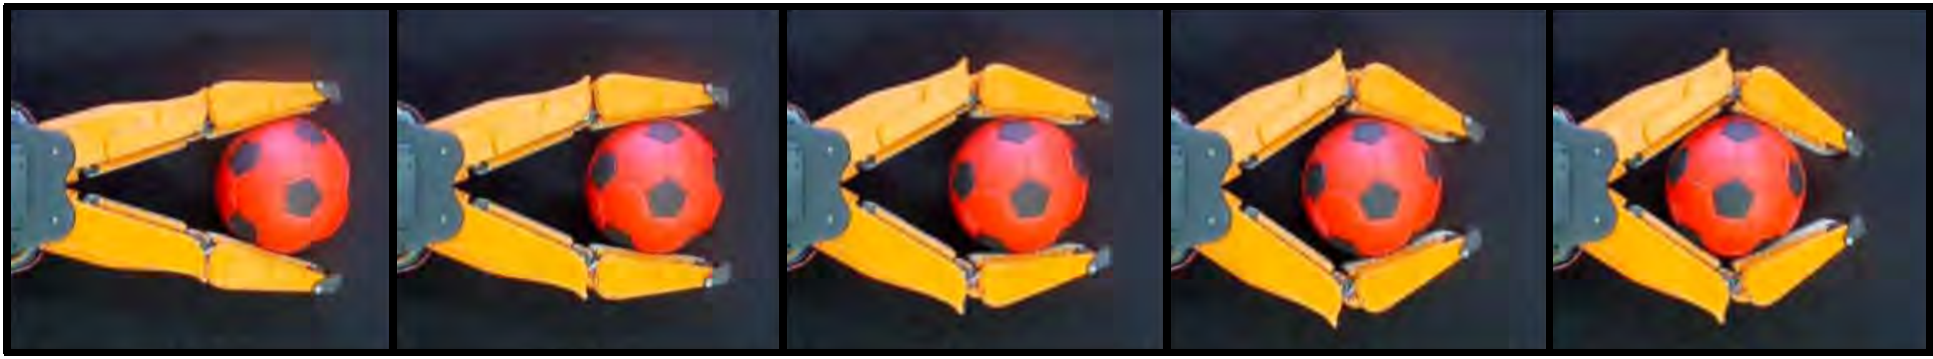
\includegraphics[width = 1.0\linewidth]{figs/pull_in}
   \caption{\textit{Pull-in grasping strategy:} Depicted is a sequence of intermediate grasp states
     where the belts of the gripper are used to pull the object towards its palm which results in a
     transition from a fingertip to an enveloping grasp.}
   \vspace{-4mm}
   \label{fig:pull_in}
   \centering
 \end{figure}
%
\begin{figure*}[!t]
 \centering
   \subfigure[]{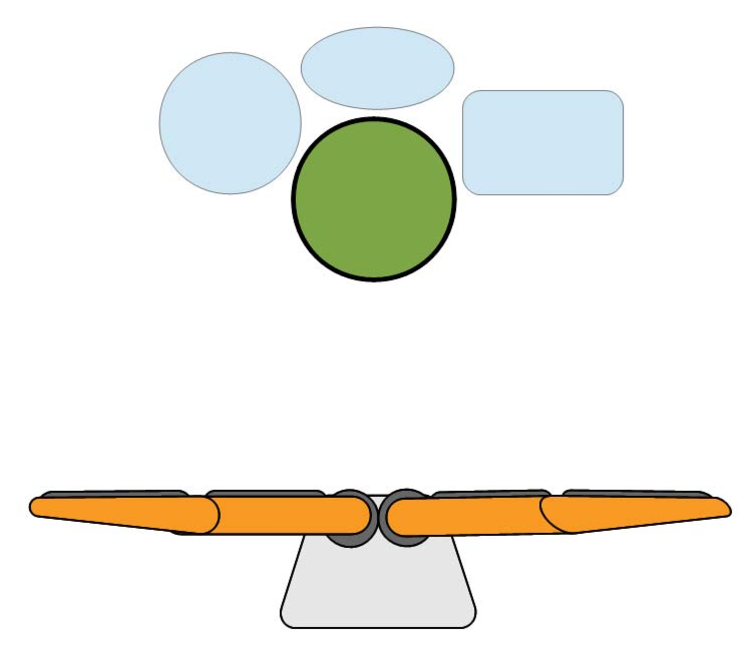
\includegraphics[width = .32\linewidth]{figs/vcg1}}
   \subfigure[]{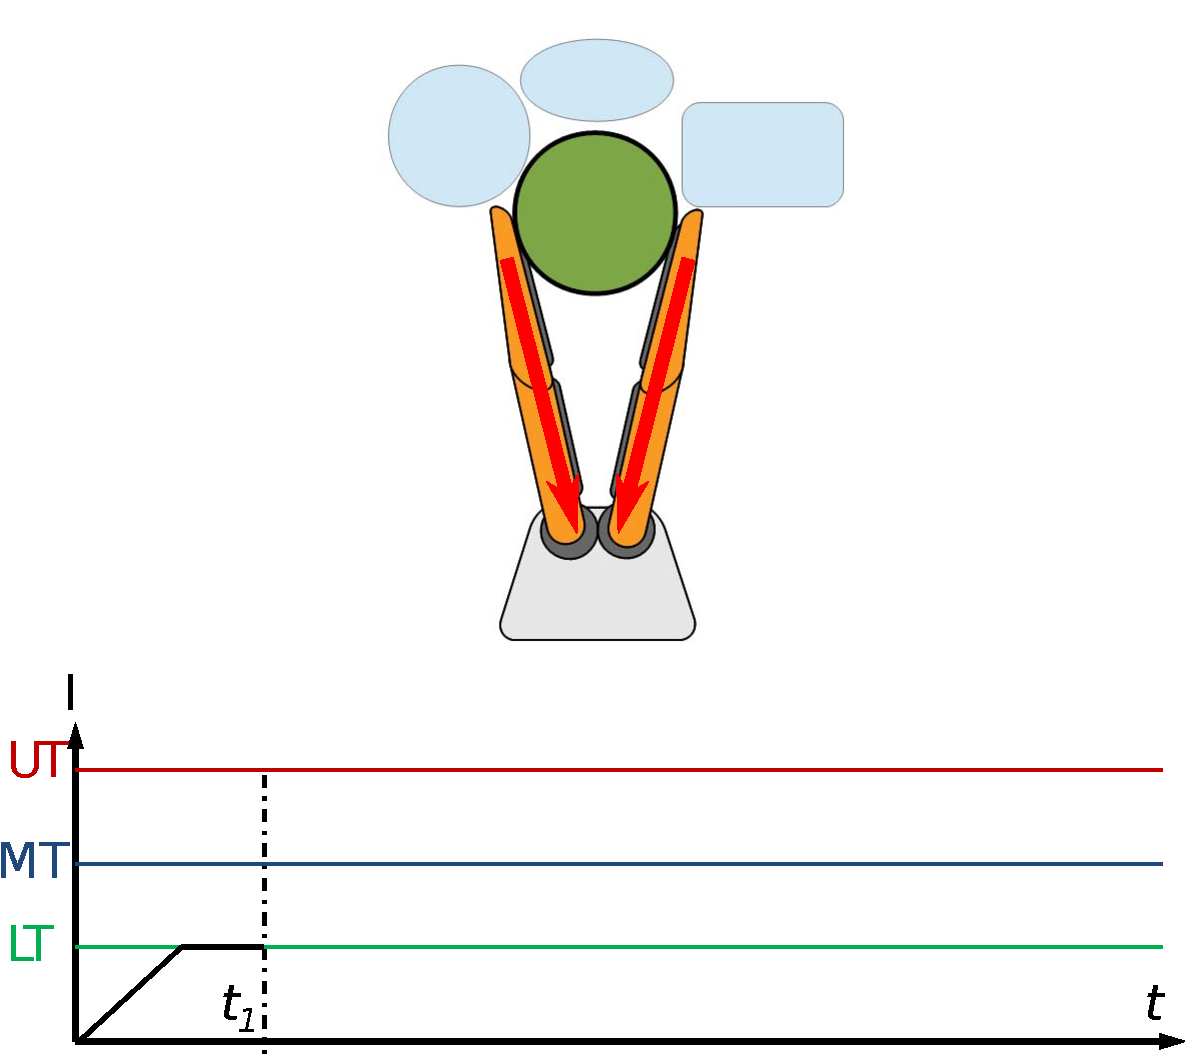
\includegraphics[width = .32\linewidth]{figs/vcg2}}
   \subfigure[]{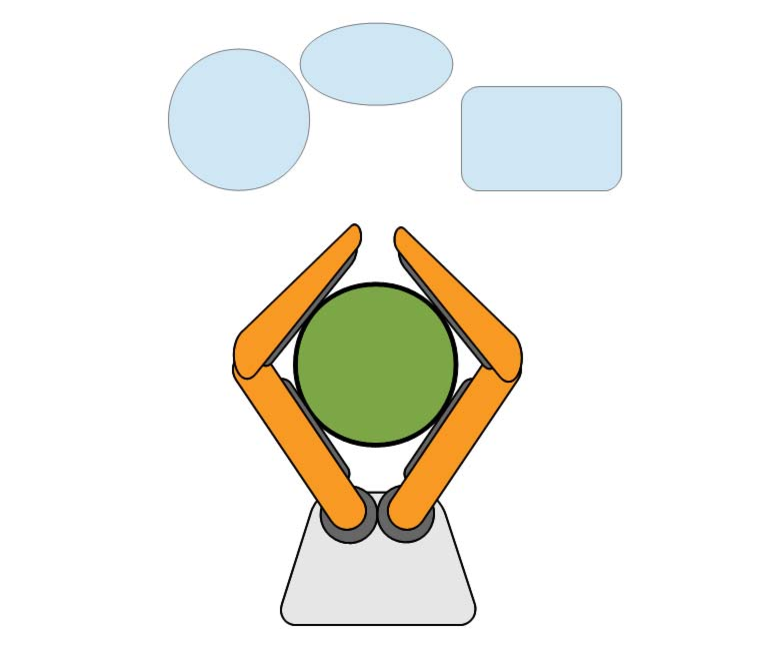
\includegraphics[width = .32\linewidth]{figs/vcg3}}
   \caption{\textit{Grasp Execution Control:} As the open griper closes in on the object (Left), the
     current through the opening motor is monitored. When contact is made (Middle), the actuated
     belts are switched on to pull in the object. The controller then strives to maintain the
     current in between two target thresholds by opening or closing the gripper during in-hand
     manipulation (Right).}
   \label{fig:pull_in_control}
 \centering
\end{figure*}
%
For this component, we leverage the capabilities of the Velvet Gripper, namely underactuation and
conveyor belts on the finger pads in order to achieve robust grasping behavior. Especially in
cluttered scenes, a ``pull-in'' strategy has been shown to be especially effective to achieve stable
grasps while starting from a relatively wide range of initial gripper poses with respect to the
target object~\cite{Krug14a}. Here, the features of the grasping device are exploited to embrace the
object in a firm envelope grasp by simultaneously squeezing it in a compliant fashion while
actuating the belts inwards.

(\hl{the following is copy/pasted from the Gripper control workshop paper})~\cite{Krug14c} Each of
the gripper’s two fingers has a planar manipulator structure with two joints and active surfaces
which are implemented by coupled conveyor belts on the inside of the two phalanges. The mechanical
structure is underactuated and comprises only one actuated Degree of Freedom (DoF) for opening and
closing and two DoF for the belt movements.  If, during grasping, the proximal phalanges are blocked
by an object, the gripper’s distal phalanges continue to “wrap around” and envelope it in a firm
grasp.  The experiments reported in~\cite{Krug14a} showed, that in cluttered scenes fingertip
grasps are more likely to be feasible than robust enveloping grasps, because the latter necessitate
large opening angles resulting in bulky gripper silhouettes for which no collision free approach
trajectories can be found. Therefore, we employ the “pull-in” strategy which is illustrated in
Fig.~\ref{nothereyet}. Here, the underactuated nature and the conveyor belts on the grasping device
are exploited to embrace the object in a firm envelope grasp by simultaneously squeezing it while
actuating the belts inwards. This is achieved by compliant low-level position controllers which
saturate on experimentally evaluated current thresholds. We use a simple grasping routine which is
triggered after an initial fingertip grasp is achieved (see Fig.~\ref{nothereyet}). This routine
consists of issuing commands to fully close the gripper while moving the belts a pre-defined offset
towards the palm. Three thresholds on the current absorption of the opening motor are used: a low
threshold (LT) signifies contact between the gripper and the object and a mid threshold (MT)
indicates a large enough contact force to stop the closing movement.  Finally, an upper threshold
(UT) prevents damage to the grasping device. Once the pull-in sequence is completed, the controllers
maintain the final torques to ensure a stable grasp.

